\documentclass[a4paper,14pt]{article}

\usepackage{comment} % Para comentar várias linhas ao mesmo tempo

%matemática
\usepackage{amsmath}
\usepackage{amssymb}

%diagramação
\usepackage{extsizes}
\everymath{\displaystyle}
\usepackage{geometry}
\usepackage{fancyhdr}
\usepackage{multicol}
\usepackage{graphicx}
\usepackage[brazil]{babel}
\usepackage[shortlabels]{enumitem}
\usepackage{cancel}
\usepackage{textcomp}
\usepackage{tcolorbox}

%tabelas
\usepackage{array} % Para melhor formatação de tabelas
\usepackage{longtable}
\usepackage{booktabs}  % Para linhas horizontais mais bonitas
\usepackage{float}   % Para usar o modificador [H]
\usepackage{caption} % Para usar legendas em tabelas
\usepackage{wrapfig} % Para usar tabelas e figuras flutuantes


%tikzpicture
\begin{comment}
	\usepackage{tikz}
	\usepackage{scalerel}
	\usepackage{pict2e}
	\usepackage{tkz-euclide}
	\usetikzlibrary{calc}
	\usetikzlibrary{patterns,arrows.meta}
	\usetikzlibrary{shadows}
	\usetikzlibrary{external}
\end{comment}


%pgfplots
\usepackage{pgfplots}
\pgfplotsset{compat=newest}
\usepgfplotslibrary{statistics}
\usepgfplotslibrary{fillbetween}

%colours
\usepackage{xcolor}



\columnsep=2cm
\hoffset=0cm
\textwidth=8cm
\setlength{\columnseprule}{.1pt}
\setlength{\columnsep}{2cm}
\renewcommand{\headrulewidth}{0pt}
\geometry{top=1in, bottom=1in, left=0.7in, right=0.5in}

\pagestyle{fancy}
\fancyhf{}
\fancyfoot[C]{\thepage}

\begin{document}
	
	\noindent\textbf{6FMA09 - Matemática} 
	
	\begin{center}Frações equivalentes (Versão estudante)
	\end{center}
	
	\noindent\textbf{Nome:} \underline{\hspace{10cm}}
	\noindent\textbf{Data:} \underline{\hspace{4cm}}
	
	%\section*{Questões de Matemática}
	
	\begin{multicols}{2}
		\noindent Duas frações são equivalentes quando representam o mesmo número. Por exemplo, $\frac{1}{2}$ e $\frac{2}{4}$ são frações equivalentes. \\
		Para simplificar uma fração, dividimos o numerador e o denominador por um divisor comum de ambos. Uma fração é irredutível quando não pode ser simplificada. \\
		\noindent\textsubscript{-----------------------------------------------------------------------}
		\begin{enumerate} 
			\item Com base na figura, complete a igualdade abaixo.
			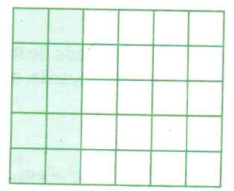
\includegraphics[width=1\linewidth]{6FMA09_imagens/imagem1}
			\\
			$\frac{10}{30} = $ \\
			\item Verifique se são equivalentes ou não os pares de frações abaixo.
			\begin{enumerate}[a)] 
				\item $\frac{6}{9}$ e $\frac{2}{3}$. \\\\\\\\\\\\
				\item $\frac{6}{14}$ e $\frac{2}{7}$. \\\\\\\\
				\item $\frac{5}{9}$ e $\frac{10}{18}$. \\\\\\\\\
			\end{enumerate}
			\item Localize, na reta abaixo, as frações $\frac{3}{4}$ e $\frac{6}{8}$. \\
			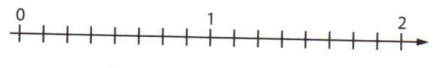
\includegraphics[width=1\linewidth]{6FMA09_imagens/imagem2} \\\\\\\\\\\\
			Você chegou a alguma conclusão? Qual? \\\\\\\\\\\\\\
			\item Simplifique a fração $\frac{24}{32}$. \\\\\\
			\item Transforme a fração $\frac{8}{52}$ numa outra fração equivalente mais simples. \\\\\\\\\\\\\\
			\item Simplificando uma fração por 9, obtemos a fração $\frac{4}{9}$. Qual era a fração original? \\\\\\\\\\\\\\
			%34 a 36
			\item Localize na reta abaixo as frações $\frac{3}{9}$ e $\frac{1}{3}$. \\
			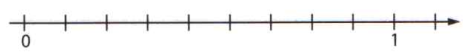
\includegraphics[width=1\linewidth]{6FMA09_imagens/imagem3} \\
			\item Assinale \textbf{V} (verdadeiro) ou \textbf{F} (falso).
			\begin{enumerate}[a)] 
				\item (~~) $\frac{4}{15} = \frac{2}{3}$
				\item (~~) $\frac{6}{8} = \frac{3}{4}$
				\item (~~) $\frac{3}{5} = \frac{9}{12}$
				\item (~~) $\frac{24}{30} = \frac{8}{10} = \frac{4}{5}$ \\\\\\
			\end{enumerate}
			\item Simplificando uma fração por 5, obtemos $\frac{3}{4}$. Qual é a fração original?
		\end{enumerate}
		$~$ \\ $~$ \\ $~$ \\ $~$ \\ $~$ \\ $~$ \\ $~$ \\ $~$ \\ $~$ \\ $~$ \\ $~$ \\ $~$ \\ $~$ \\ $~$ \\ $~$ \\ $~$ \\ $~$ \\ $~$ \\ $~$ \\ $~$ \\ $~$ \\ $~$ \\ $~$ \\ $~$ \\ $~$ \\ $~$ \\ $~$ \\ $~$ \\ $~$ \\ $~$ \\ $~$ \\ $~$ \\ $~$ \\ $~$ \\ $~$ \\ $~$ \\ $~$ \\ $~$
	\end{multicols}
\end{document}